%% Support sites:
%% http://www.michaelshell.org/tex/ieeetran/
%% http://www.ctan.org/tex-archive/macros/latex/contrib/IEEEtran/
%% and
%% http://www.ieee.org/
%****************************************************************

\documentclass[pdf,bookmarks,colorlinks=true]{IEEEtran}
\usepackage{times}
\usepackage{amsmath}
\usepackage{hyperref}
\usepackage{url}
\usepackage{psfrag}    %Shouldn't use this if you plan on using pdflatex!
\usepackage{graphicx}
\usepackage{wrapfig}   %for wrapping text around figures and tables
\usepackage{graphicx}

\makeatletter
\def\endthebibliography{%
	\def\@noitemerr{\@latex@warning{Empty `thebibliography' environment}}%
	\endlist
}
\makeatother

\begin{document}
%
% paper title
% can use linebreaks \\ within to get better formatting as desired
% Do not put math or special symbols in the title.
\title{Review of Cybersecurity in the Radiology Department}


\author{Leonardo Arthur Pangemanan\\
	Southern Adventist University\\
	lpangemanan@southern.edu
}



% The paper headers
\markboth{CPTE-542-A Survey Paper, October 2019}%
{Shell \MakeLowercase{\textit{et al.}}: CPTE-542-A Survey Paper, October 2019}

\maketitle

% As a general rule, do not put math, special symbols or citations
% in the abstract or keywords.
\begin{abstract}
	Cybersecurity is an increasing concern for many healthcare organizations, information technology and medical cybersecurity professionals. As more computerized medical devices become connected to the network within and outside the facility increases, the risk of cyber attacks also increases. Moreover, the radiology departments have most of their devices connected to the network. Most radiologists are unaware of the vulnerability of their devices. This paper will review the cyberthreat of modern medical devices within the radiology department to build more awareness to these vulnerabilities.
\end{abstract}

\section{Introduction}
\IEEEPARstart{T}{he} healthcare industry has change ever since the first computer were introduced. The healthcare technologies have the potential to extend, save and enhance the live of patients. Furthermore, hospitals have witnessed a proliferation of networked medical equipment in the past decade. There is an emergent trend of connecting medical equipment to the hospital network for easy accessibility and manageability. As healthcare devices continue to evolve, so does the inter-connectivity. For example, it provides efficiency, error reduction, automation, and remote monitoring. Interconnected technology allows health professionals to monitor and adjust devices without the need for hospital visit or invasive procedure \cite{coventry2018cybersecurity}. With integration comes complexity and challenges in management and this protection \cite{williams2015cybersecurity}. However, interconnected technology introduces new cybersecurity vulnerabilities in the same way other networked computing systems are vulnerable. Recently, securing medical devices against cyber attacks or malware outbreaks and safeguarding protected health information (PHI) stored on devices or exchanged between a device and the provider's network is a growing challenge for clinical engineers and hospital information technology (IT) professional \cite{wirth2011cybercrimes}. The number of high-profile public demonstrations of successful attacks on devices and medical networks have increased. This fact raises the concern that inter-connectivity will directly affect clinical care and patient safety. \par
% New Paragraph
Over the past few years, the question of inadequate clinical security has been gaining attention from both industry leaders and clinical practitioners. The integration of medical devices, networking, software, and operating systems means that the relative isolation and safety of medical devices are challenged \cite{williams2015cybersecurity}. These vulnerability is also due to many manufacturers focus their efforts on innovation and functionality, with little emphasis on the network security of this devices \cite{moses2015lack}. \par
Designing a secure medical device is fundamentally different from  any other devices that only focus on safety and efficacy. Safety design decisions are based on the assumption that hazardous condition or failure occur accidentally. However, the assumption that hazardous condition or failure occurs accidentally no longer holds true as malicious attackers try to trigger hazards in devices through intentional repeated attempts \cite{Ray}. Thus manufacturer tends to not implement the necessary security check against these malicious attacks. This fact become more important as the radiology departments usually have the highest density of networked medical equipment in a hospital \cite{moses2015lack}. 

The rest of this paper first discusses the background of cybersecurity in
\ref{sec:Background}, and then describes my main topic in
\ref{sec:Radiology}. Lastly, \ref{sec:Conclusion} presents the
conclusions and describes future work.

\begin{table*}[tbh]
	\caption{Common cyber threats in healthcare \cite{martin2017cybersecurity}.}
	\centering
	\begin{tabular}{l | l}
		\hline
	Data theft for financial gain & Stealing personal data for the purposes of monetary gain. \\
	Data theft for impact & Theft and public release of sensitive medical information. \\
	Ransomware & Using malware to block users from their data or systems or to delete data unless a fee is paid. \\
	Data corruption & Deliberate corruptions of data, such as altering test results, for political or personal gain. \\
	Denial of service attacks & Disruption of a network or system by flooding it with superfluous requests motivated by blackmail, revenge, or activism. \\
	Business email compromise & Creating fake personal communications for financial gain.\\ 
	The unwitting insider & Substantial disruption to systems or the loss of data owing to the unintentional actions of staff using outdated and at-risk systems. \\
	\hline
	\end{tabular}
	\label{tab:common}
\end{table*}

\section{Background}
\label{sec:Background}
With the numerous data breaches in healthcare over the last several year, it seems to be unreasonable for patients having any expectation of privacy and security in their health information. In 2012, 780,000 patients records were stolen from the State of Utah Department of Health, Department of Technology server, by an Eastern European hacker. Another at Saint Joseph's Health System in California, approximately 31,800 patients' record was made potentially available through basic Internet search engines for about a year because security settings on the system were set incorrectly \cite{murphy2015cybersecurity}. Increasingly, healthcare is a prime target for cyber attack with a recent SANS Institute report reporting that 94\% of healthcare organization have been the victim of a cyber attack \cite{williams2015cybersecurity}. Table \ref{tab:common} shows the most common cyber attacks healthcare organizations is vulnerable to. In May 2017, a ransomware called WannaCry infect more than 200,00 computers in 150 countries. One of the victim was the National Health Services (NHS) in the United Kingdom. Nearly 19,000 appointments had to be canceled, costing them and estimate \pounds20 million. The NHS spent an additional \pounds72 million to recover from the disaster and upgrade its systems \cite{ferrara2019cybersecurity}. The vulnerability of healthcare to cyber attack reflects a combination of factors, notably limited resources, fragmented governance, and cultural behavior. \par
In May 2017, The Ponemon Institute shared a survey that showed only 15\% of healthcare delivery organization (HDOs) and 17\% of medical device manufacturers (MDMs) were taking significant steps to prevent cyber attacks \cite{busdicker2017role}. Figure \ref{fig:total-number-of-malware-per-year} shows the total number of malware that is on the internet. With this many malware, there should be a protection against them. However, most healthcare organization exist to provide cybersecurity within their devices. The industry more focuses on providing healthcare to the patients in need. Their revenue or reimbursement for healthcare is not tied to any cybersecurity effort. More importantly, there is a traditional believes that no one would be motivated to attack healthcare systems and protective measure were not necessary. As mentioned before, many of these healthcare organization ignore the potential danger of cyber attack and solely focus on giving patient care \cite{coventry2018cybersecurity}. Moreover, the healthcare industry is one of the most targeted sectors globally; 81\% of 223 organizations surveyed, and $>$110 million patients in the United States had their data compromised in 2015 \cite{martin2017cybersecurity}. Currently, there are many motivations for hackers to attack healthcare organizations and professional needs to increase the priority to enhance their cybersecurity.

\subsection{Cybersecurity Terminology}
Cybersecurity terms are unfamiliar to many people and can leads to misunderstanding by those who do not work in the cybersecurity or information technology professions. Here are some of the most common terms associated with cybersecurity based on \cite{ferrara2019cybersecurity}:
\begin{itemize}
	\item {\bf Distributed Denial of Service (DDoS)}: A cyber attack where the hacker use multiple device to send a request to a website or a network. If the number of requests is large enough, the website or network cannot handle the traffic and stop responding, therefore preventing legitimate users from accessing the network.
	\item {\bf Malware}: Typically a software designed to interfere with the computer's normal function. This interference can take the form of destruction of data, inability to run the computer or certain programs, stealing personal information, or causing physical damages to the device. Figure \ref{fig:total-number-of-malware-per-year} shows the yearly total number of Malware that has been developed in the past ten years. The different types of malware include:
	\begin{itemize}
		\item {\em Ransomware} - Malware that encrypts all file on a device, making them unreadable and inaccessible.
		\item {\em Virus} - Section of computer code that adds itself to files and spread in one computer and to other computers. Ransomware is a type of virus.
		\item {\em Trojan} - A program that seems legitimate but are, in fact, malicious. Trojan allows hacker to access the infected device unnoticed and steal personal information or to steal passwords.
		\item {\em Worm} - A standalone program that spreads among computers but does not infect individual files.
	\end{itemize}
	\item {\bf Phishing}: Emails that pretend to be from official entity. These emails usually contains a link or attachment that are malicious. The goal is steal sensitive information, such as financial institution login credential.
	\item {\bf Virtual Private Network (VPN)}: A VPN allows users to connect to a private network securely, even when the connected network are not private (e.g., free internet connection at a coffee shop).
	\item {\bf Vulnerability}: A weakness in software or hardware. When a vulnerability is discovered, manufacturer should release a patch or fix to eliminate the vulnerability.
\end{itemize}

\subsection{Implantable Medical Devices}
\emph{Implantable Medical Devices} (IMDs) apply continuous monitoring and automatic therapies to the treatment of chronic medical disorders \cite{Rostami:2013:HAI:2541806.2516658}. For example, a typical IMDs monitor and treat physiological conditions within the body and improve patients' quality of life and help sustain their lives.  These devices includes pacemakers, implantable cardiac defibrillators (ICDs), drug delivery systems, and neurostimulator. With these devices, health professional can treat abnormal physiological conditions within the body, such as cardiac arrhythmia, diabetes, and Parkinson's disease. IMDs' pervasiveness continues with upward of 25 million United States citizens currently reliant on them for life-critical functions \cite{halperin2008security}. In the United States, over 100,00 patients a year receive implantable cardioverter defibrillators (ICDs), which detect dangerous heart rhythms and administer electric shocks to restore normal activity \cite{Rostami:2013:HAI:2541806.2516658}. Some current-generation devices now have the ability to communicate wirelessly with external equipment from distances up to five meters away \cite{denning2010patients}. In fact, the latest IMDs is able to support remote monitoring over long-range, high-bandwidth wireless links, and emerging devices will communicate with other inter-operating IMDs. \par
Despite these advances in IMD technologies, they still can occasionally malfunction. Additionally, they are still behind in security and privacy. Many information technology professionals are still lacking in the understanding of how device security and privacy interact with and affect medical safety and treatment efficacy. Cybersecurity protection of these devices are not just a technical issue according to \cite{williams2015cybersecurity}. The foundational study of these devices demonstrated the vulnerability is detrimental to their safe operation, and the availability, confidentiality, and integrity ot the associated data. IMDs poses the challenge of having a balance of security and accessibility for medical professionals.	

\begin{figure*}[tbh]
	\centering
	\includegraphics[width=0.7\linewidth]{"Total Number Of Malware per Year"}
	\caption{A graph of total number of Malware per year, based on data from AV-TEST \cite{AVtest}.}
	\label{fig:total-number-of-malware-per-year}
\end{figure*}


\section{Cybersecurity in Radiology Department}
\label{sec:Radiology}
Healthcare today increasingly depends on computers, networking, and information system. Due to the need of digital healthcare, most diagnostic imaging systems are connected to the Internet/LAN (Local Area Network) \cite{ma2019medical}. Furthermore, this connectivity enables computer enhanced medical imaging capabilities, that allows for early discovery of diseases, research new diseases, and better treatment of medical condition. Additionally, this improvement enables doctors extracting meaningful information from patients' digital records. It would permit doctors to detect and then treat a disease at its earliest stages. Increasing the quality of medical services \cite{Marwan}.
Further, the radiology department have seen a more proliferation of networked equipment in the past decades. They also have the highest density of networked medical equipment. However, many manufacturers focus solely on innovation and functionality but little effort was put on the network security of this equipment. For example, radiologist uses a system called Picture Archiving and Communication System or Radiography Information System (PAC/RIS) \cite{ferrara2019cybersecurity}. It is a technology that provides doctors with economical storage and convenient access to image from multiple source machine types. PACS receive images from medical imaging devices through an acquisition gateway. From the acquisition gateway, the images is moved to the database system, where they are archived. This eliminates the need to manually file, retrieve, or transport film jackets, the folders used to store and protect X-Ray film. With the development of PACS/RIS, traditional diagnostic imaging system have been replaced to computer assisted ones. Further, the universal format for PACS is Digital Imaging and Communications in Medicine or DICOM \cite{InformationSecurityonDiagnosticImagingSystem}. DICOM is an international standard to transmit, store, retrieve, print, process, and display medical imaging information. This digital storage and transmission of images across the hospital network using PACS technology have become a well-established norm in most large radiology departments \cite{moses2015lack}. With this increase of connectivity imaging devices, the issue of cybersecurity is now involves more than just the security and integrity of patient data and machine operation. \par 
There is a common term used in medical device cybersecurity that is called CIA (or CIA triad), which stands for the categories confidentiality, integrity, an availability. Confidentiality refers to protecting patients' information and ensuring that data are always available to people with legitimate needs. Integrity means preventing malware from altering patients' medical information. Availability means the data, the device, the network, and  the operations software are always accessible and available \cite{mahler2018know}. 
However, with all of these advancement of technology, a breach of security on one computer can bring down the entire hospital's network, compromising patient care and putting patients at risk of harm, threatening their confidentiality, safety, and well-being \cite{ferrara2019cybersecurity}. Something have to be done to eliminate this security issue.

\subsection{Diagnostic Imaging System}
Diagnostic imaging (DI) system is a technique that creates visual representation of the interior of a body for clinical analysis and medical intervention -- for example magnetic resonance imaging (MRI), X-Ray, ultrasound, computed tomography (CT), and positron emission tomography (PET) \cite{InformationSecurityonDiagnosticImagingSystem}. Almost all of these devices uses PACS to store the data information and DICOM to transmit the data across the networked devices. All of these connection between the different diagnostic imaging system makes them more vulnerable to networked related cyberthreats. DI systems are used extensively all the time, and for various reasons such as supporting life-saving treatments. These devices are a critical resources because of the expensive cost to maintain one, thus, very few of them are held by hospitals. Therefore, failure of one device may sabotage entire hospital's operation \cite{mahler2018know}. This fact added with several motivations for malicious hackers to target medical imaging devices, can have a disastrous consequences that may cost millions of dollar to recover from.

\begin{figure*}[tph]
	\centering
	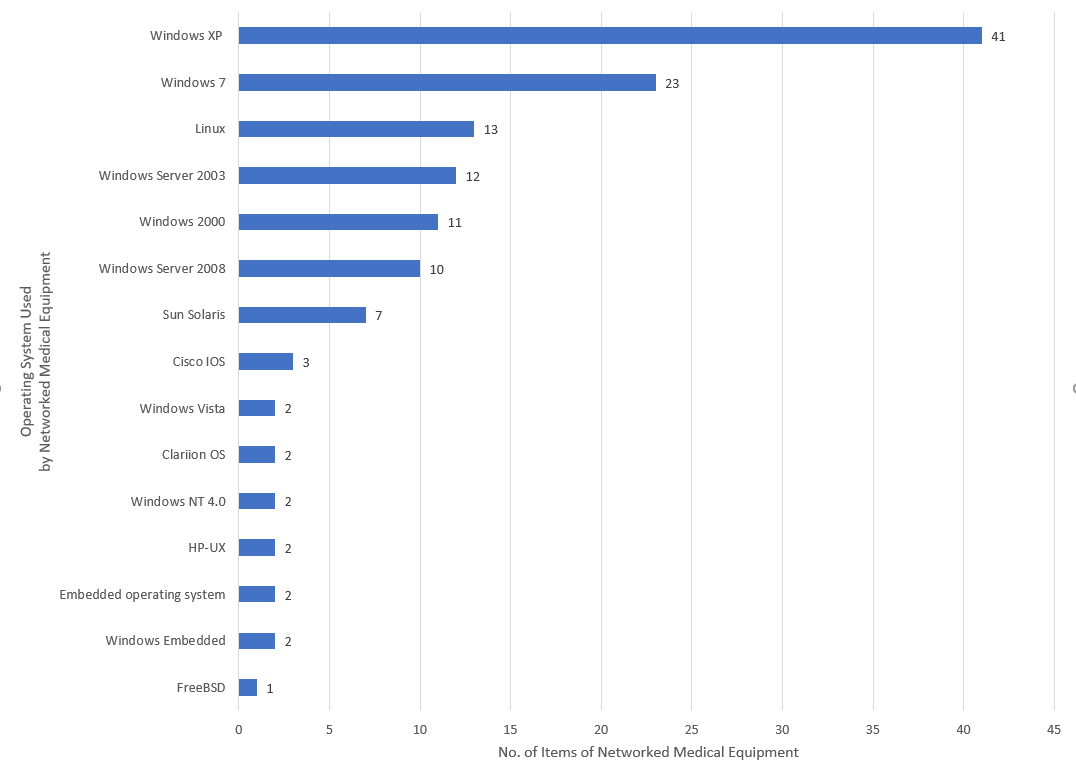
\includegraphics[width=0.7\linewidth]{OSonRadiology}
	\caption{The distribution of Operating System running on networked medical equipment in the radiology department \cite{moses2015lack}.}
	\label{fig:osonradiology}
\end{figure*}

\begin{table}[tbh!]
\caption{Top 10 Countries with Open DICOM Servers \cite{stites2016secure}.}
\label{tab:DICOMServers}
\centering
\begin{tabular}{|c|c|c|}
	\hline 
	\multicolumn{3}{|c|}{Absolute No. of Open DICOM Servers} \\ 
	\hline
	Rating & Country & No. Of Servers \\ 
	\hline 
	1 & United States & 346 \\ 
	\hline 
	2 & Brazil & 51 \\ 
	\hline 
	3 & Turkey & 49 \\ 
	\hline 
	4 & Iran & 34 \\ 
	\hline 
	5 & India & 28 \\ 
	\hline 
	6 & South Korea & 15 \\ 
	\hline 
	7 & Taiwan & 14 \\ 
	\hline 
	8 & Mexico & 14 \\ 
	\hline 
	9 & Canada & 13 \\ 
	\hline 
	10 & Australia & 12 \\ 
	\hline 
\end{tabular}
\end{table} 

\subsection{Vulnerabilities Found in the Radiology Department}
A recent worldwide security sweep of DICOM servers found more than 2700 networks that were not secured. A research was conducted by McAfee to find vulnerability on DICOM and PACS used by medical facilities of all sizes \cite{McAfee}. As mentioned above, PACS operates on acquisition gateway to receive images. This acquisition gateways usually are placed in the facility's computer network instead of being insulated from it. Although it is done to increase efficiency, this leaves the gateway vulnerable to attacks and potentially compromises patient confidentiality. PACS price ranges from free (open-source PACS)to exceedingly expensive. Many smaller facilities favor more towards free PACS to cut expenditure. The problem with free open-source PACS is that it runs on old software platform that contains multiple vulnerabilities. Many of these PACS system are based on Windows XP, even though Microsoft announced the end of support for Windows XP in 2014 \cite{ma2019medical}. Furthermore, the researchers found 1100 unprotected PACS servers that directly connected to the internet around the world. They also were able to obtain the server name and version number the PACS was built on. \par 
The fundamental standards running contemporary digital medicine, DICOM, were conceived and developed in the late 1980s. Despite being the standard for more than 20 years, the security part was nearly untouched. There was some later standard changes and legal reinforcements; However, the medical data security has never been soundly built into the clinical data or devices, and is still largely theoretical and does not exist in practice  \cite{ferrara2019cybersecurity} \cite{ma2019medical} \cite{stites2016secure}. Furthermore, many researcher did a vulnerability scanning on the DICOM server worldwide. Table \ref{tab:DICOMServers} shows the finding of Nmap scan result. Unfortunately, the country with the most prevalent DICOM rating also tend to lead in the most unsecured DICOM rating. In the United States, there is 346 number of servers that is open with no protection. This fact implies that patients in the United States have the highest risk of having their medical records stolen or compromised \cite{stites2016secure}. Then, Figure \ref{fig:osonradiology} gives a distribution of the heterogeneous composition of operating systems running on the radiology network. Most of the equipment used Microsoft Windows, and the next largest subnet running Unix or Linux. Among the equipment running on Windows, a significant portion ran Windows XP with Service Pack 2; Service Pack 3 and the security updates released subsequently had not been installed on these machines. The other equipment running different version of Windows is not been updated with the latest service pack or security update \cite{moses2015lack}.  Additionally, another researcher, McAfee, discovered thousands of data available for download, many of them containing protected health information such as patients' names, ages, weight, facility, and city where the imaging study was done. They combined PACS and DICOM vulnerabilities to create a fictitious patient record, complete with a knee radiograph. They later penetrated the server again and changed all references in the record from the knee to elbow. The change was successful and saved in the fictitious patient's record \cite{ferrara2019cybersecurity}. In the end, this research was done with the intention to help. The McAfee researchers notifies all the vendors whose vulnerabilities they exploited from their finding and are working together to overcome these deficiencies  \cite{McAfee}. On a side note, another big vulnerability of medical imaging devices is the reliance on portable storage media, such as universal serial bus, or USB, drives. Patients and care providers often bringing imaging scan results to the health delivery organization on portable media, which are not secure and can easily be infected with malware \cite{ferrara2019cybersecurity}. 

\subsection{Effort to Improve Cyberecurity}
Many researcher and information technology professionals try to make a secure systems for the healthcare industry. For example, \cite{Almohri:2017:TMM:3204094.3204113} made a threat modeling and mitigation of medical cyber physical systems. In December 2016, the FDA published nonbinding recommendations. the draft guidance intentionally does not prescribe any particular approach or technology but instead recommends that manufacturers to consider cybersecurity at the early phase of development of the medical device. The FDA recommends that manufacturers provide \cite{fu2014controlling}: 
\begin{itemize}
	\item A specific list of all cybersecurity risk that were considered in the design process of a device.
	\item A specific list and justification for all cybersecurity controls.
	\item A traceability matrix that links actual cybersecurity risk.
	\item The systematic plan for providing validated updates and patches to operating systems or medical device software.
	\item Appropriate documentation to demonstrate that the device will be provided to purchasers and users free of malware.
	\item Device instructions for use and product specifications related to recommended antivirus software and/or firewall. 
\end{itemize}
Although the FDA acknowledges the need to consider cybersecurity throughout the life cycle of a medical device, these guidance documents are not enforceable by law. This recommendation to manufacturers is not enough to keep the radiology department cybersafe. Cybersecurity training should be mandatory for all employees of a health delivery organization, regardless of their role in the organization \cite{ferrara2019cybersecurity}. Lastly, there should be a matching between the lifecycles of underlying software to the production lifecycles of the medical device. For example, if a component is known to have a limited lifetime, then the medical devices using that component run the risk of inheriting the limited lifetime \cite{fu2014controlling}.

\section{Conclusion}
\label{sec:Conclusion}
Modern healthcare delivery is depended on medical device software to help patients lead more normal and healthy life. The cybersecurity issue with medical devices is real, but the focus on solving the issue is still lags behind. As a consequence, many medical devices is highly vulnerable at a time when it is increasingly becoming a high value target for malicious hackers. Furthermore, network breaches and vulnerability findings should be the driving force to increase the protection of medical devices. Patients should not worry about their medical records being compromised. Health professionals should be trained regularly about the importance of cybersecurity. \par 
In summary, the technological shift in medical device manufacturers and health delivery organizations is required to better deter and prevent cyber attacks on medical devices. More collaboration between the two is needed to established a foundation where many medical devices can operation without being compromised and enables efficient, high-quality patient care.


%--- bibliography ---
\bibliographystyle{IEEEtran}

\bibliography{reference}
% that's all folks
\end{document}


